\newcommand{\pc}{ProcessCache\xspace}
% Name we give to our "cachable units".
\newcommand{\cacheunit}{exec-unit\xspace}
% Lines of Code for P$
\newcommand{\systemLOC}{ProcessCache\xspace}

\chpt{\pc: Automatic Process-Level Memoization}
\label{chap:processCache}
This chapter is an updated and revised version of our current \pc draft, meant to be published at a future conference. Figures and writing are entirely written by Kelly Shiptoski and myself in collaboration.
\section{Introduction}
Existing systems already attempt to skip unnecessary recomputation. At the language-level, a runtime may attempt cache previously computed results, a technique known as memoization. This technique is most popular in purely functional programming languages like Haskell, where one can statically determine the IO and side effects of a function. Futhermore, programmers may implement their own memoization or caching in an ad-hoc manner for performance gains.

Build systems like Make \cite{make} and Bazel \cite{bazel} also skip unnecessary rebuilding when it determines none of the input sources to a build target have changed. The user must manually specify the input sources to a build step and the output build artifacts. Under-specifying or over-specifying dependencies or outputs can lead to erroneous builds \cite{perfect-dependencies}, and the all too common need to \code{make clean} when software builds are not properly updating. Forward build systems \cite{forward-build-systems} like Rattle \cite{rattle} attempt to avoid these issues by automatically inferring build dependencies and build targets.

Incremental computing aims to only recompute what is strictly necessary when inputs have changed, thus saving computing time and energy. This technique can be implemented at the language level \cite{incremental-computing} or as a language-level framework/library \cite{salsa}. Incremental computing can be combined with stream processing for low-latency result updates \cite{naiad}. 

\section{Caching/Memoizing Computation}
We generalize exisiting ideas of caching and memoization to work at the whole-program granularity. We take a systems approach to avoiding unnecessary recomputation.

In this paper, we introduce \pc a system for automatically skipping unnecessary recomputation. \pc automatically determines all inputs an outputs to a computation and caches the results of any computation it has no seen before. Whenever the same program is executed with the same inputs, \pc skips the actual execution of this program and uses the cached results instead. \pc can be thought of as a general purpose make-like system, except no \code{makefile} is required and works on diverse sets of programs beyond build system. 
 
Linux utilizes the \code{execve} system call to launch a new process image. This is the standard way
a program is launched. We refer to a \textit{program} as the root command that \pc will execute on.

\pc parses the command line arguments passed to it and attempts to \code{execve} the given program.
\code{./process \textunderscore cache [process cache params] -- <exe> [exe params]}
A program is comprised of possibly many processes, those processes may themselves spawn new child processes and contain multiple threads, any child process may further call \code{execve} spawning new sub-programs. See Figure \ref{fig:exec-units} for details. The root \cacheunit{} will always exists, as it is created by \pc based on the CLI arguments as
described above.

We use a unique key to uniquely identify every program \ref{sec:unique-program}. Whenever \pc sees a call to
\code{execve}, it checks the program specified by the system call. \pc does a lookup in our cache, a cache hit means we have seen this program before. The cache contains the outputs of this program. Instead of executing
the program, \pc copies the output file and write the correct output to stdout and stderr. \pc essentially skips running the program but still produces the correct output of the program.

\subsection{Detemining Program Inputs}
Modern programs have many explicit but also implicit inputs. Explicit inputs include: command line arguments,
input files, interactive input via stdin, network connections, pipes, etc. Implicit inputs include: any configuration files ready by the program, reading bytes from the network, environment variables.

Any state that could affect the execution of the program could be considered an input. Some of these inputs
may not be so obvious, such as file metadata, time, signals, etc.

\pc relies on the assumption that program output is a deterministic function of its inputs, see section \ref{determinism}. By considering all the inputs to a program we can define a unique program execution
as the combination of the program binary and all of its inputs. As long as none of the program inputs have changed, it is safe to skip reexecuting a program, and simply use the cached results.

For correctness, \pc attempts to consider as many inputs to a program. \pc must know be able to observe
all program inputs at "exec-time" to determine if any program input has changed. This is the main criteria for deciding which inputs \pc considers: an program input must be observable before the program is executed. 


\subsection{Determinism} \label{determinism}
\pc operates under the assumption that if a program is executed multiple times, with the same program
inputs, it will produce the same outputs, that is, the program executes \textit{deterministically}.

In practice this is not always the case due to various sources of non-determinism that sneak in \cite{dettrace}. \pc is compatible with the orthogonal work on dynamic determinism enforcement at various levels. However,
\pc does not require a program to be deterministic or to use a dynamic enforcement mechanism to produce correct output. When \pc encounters a never before seen program plus inputs combination, it captures the results of this program. This is a valid result for this program, subsequent executions of this program and inputs will be skipped and the cached results will be used instead.

This works around issues of nondeterminism from thread and process scheduling, etc.

As long as we consider all inputs (even tricky ones like time) to a program, it is valid to cache and skip. \pc could be combined with other systems like Dettrace, Arnold \cite{arnold}, Dthreads \cite{dthreads}, if you do not like our approach.

\subsection{Handling Program Side-Effects}
A pure program would have no observable effects.

An effectful program will have some observable behavior on the system. Most commonly, a program will make
changes to the filesystem, such as modifying, deleting, or writing to files. Write to stdout or stderr.
A program may also write bytes to the network, or display results on the terminal or a graphic user
interface.

Any obeservable change to the state of the world is known as a program side effect. To effetively simulate
a program being skipped with \pc we must be able to perform the same side effects a program would have done. \pc handles common side-effects seen in batch workloads: writing to output files: stateful changes
to the filesytem.

\pc does not support networking. There is a long list of possible side effects a Linux program may
support which are not implemented due to too much engineering effort, these include: sending signals,
creating FIFOs, or many OS operations. These are not fundamental shortcomings of our design however, and can be implemented into our prototype with more engineering effort.

\subsection{Correctness}
When skipping, any caching system like \pc should give the same results as if the computation was to actually be executed. \pc is able to skip redundant programs and only re-execute programs whose inputs have changed.

As an example consider make. Running make from a "clean" state with no build files will force all build
rules to execute. Future runs of make will only execute the build rules where an input has changed. We expect make to produce the same results after a "make clean" versus running "make" and allowing make to automatically skip unnecessary re-computation. This property is known as from-scratch-consistency.

\pc is designed in such a way to always maintain correctness. \pc introspects all relevant IO
events a program executes. So it is always able to precisely determine all actions required to later
emulate the execution of the program. When \pc detects IO events it cannot handle and skip, e.g. writing bytes to the network, sending signals to other processes, ioctl, \pc can always maintain correctness by simply choosing not to skip the program and falling back to executing it.

\section{\pc Design}
We present \pc, a system to automatically cache and skip unnecessary reexecution of computation. By tracking program input and outputs, \pc is automatically able to detect redundant computation. The next time the same exec is executed, \pc checks if any input has changed. If no input has changed, we can skip re-executing the \cacheunit{} and simply re-execute the program side-effects. An external observer should not be able to determine whether \pc actually executed a \cacheunit{} or skipped it, save for a noticeable speed-up of execution time.

\pc is able to skip entire "exec trees", that is, programs made of multiple calls to processes and execs.
\subsection{Determining Granularity of Memoization Units}

\begin{figure*}
\centering
\subfloat[]{
    \label{fig:single-exec-unit}
    \includegraphics[scale=0.5]{"pc_single_exec-crop.pdf"}
}
\subfloat[]{
\includegraphics[scale=0.4]{"pc_multi_process-crop.pdf"}
}
\subfloat[]{
\label{fig:multi-exec-unit}
\includegraphics[scale=0.25]{"pc_multi_exec-crop.pdf"}

}
\caption{The \cacheunit{} provides a useful abstraction over diverse program fork-exec structures. Processes are represented by darker circles with the letter P. Threads are represented by lighter
circles with the letter T. (a) In the simplest case, a program contains one \cacheunit{} with one process. (b) An exec-unit may internally contain multiple processes and those processes may be multi-threaded. (c) A program containing multiple \cacheunit{} with their own possibly complex internal
structure.}
\label{fig:exec-units}
\end{figure*}

We consider several candidates for cache-unit. A cache-unit is the smallest "unit of work" any system in this space may consider for caching and skipping. These can be small like regions of instructions. They can be domain specific like compilation-units for build systems, or entire programs. So, what is the right granularity of computation to cache? We consider several factors:

\begin{compactitem}
  \item Size of cache-unit.
  \item Ease of tracking cache-unit inputs.
  \item Number of opportunities to skip cache-unit
\end{compactitem}

At one extreme end, we could cache and skip an entire program, but then any changes to an input would force us to reexectue the entire program, so our skipping wouldn't be very useful. On the other end of the spectrum, there are systems like Shortcut \cite{shortcut} which are able to skip "mostly-deterministic" regions of code. Shortcut is able to skip chunks of program instructions at a time. Shortcut's approach provides considerable opportunities to possibly skip, but this comes at the cost of complicated low-level machinery to track inputs and skip instruction-level computation.
It is natural to consider the process as a candidate for our caching-unit. In a multi-processed program, we could then skip unnecessary processes, only executing those whose input has changed. Processes are difficult however. A cache-unit should be uniquely identified by its inputs, for a Linux process, the starting input
  includes the entire state of the parent process from which our process was forked/cloned from. This "input" process-image state is difficult to track. 
Instead, \pc uses the Linux \code{execve} system calls as our cache-unit. \code{execve} provides several advantages to caching. Unlike processes, execs have clear inputs: an exec can
be uniquely identified by a tuple containing the: binary executable, command line arguments, environment variables, and any IO inputs read at runtime. This allows us to quickly and easily check if a \cacheunit{} needs
to be recomputed (one of its inputs has changed) or can be skipped.

Other benefits:
\begin{compactitem}
  
  \item Many Linux programs are written in a "fork-exec" style of computation. So execs provide a natural
  cache-unit.
  \item This design naturally supports multi-process execs (one exec call which spawns multiple processes) and multi-threaded programs. We only consider the execs and implementation details of a program like number of processes, threads, pipes, etc are abstracted over.
\end{compactitem}

\subsection{The \cacheunit}
\pc works at the granularity of \cacheunit. \pc caches the results of \cacheunit{} and at every exec
IO event, determines whether it can skip this \cacheunit. Figure \ref{fig:single-exec-unit} show the simplest
case for a program: a single exec-unit containing one process. The \cacheunit{} abstracts over the process and
thread structure of a program. Just like processes form a natural tree structure for programs, \cacheunit{} also
create a tree structure as shown in Figure \ref{fig:multi-exec-unit}. Every individual \cacheunit{} in Figure \ref{fig:multi-exec-unit} is a candidate for skipping. Furthermore, \pc can also cache entire \cacheunit
trees or subtrees.

Programs with a fork-exec structure are the best candidates for \pc, as this creates the most candidate \cacheunit{} for skipping. Many Linux workloads follow the fork-exec paradigm, making our \cacheunit{} a natural choice.

\subsection{Tracing Program IO Events} \label{sec:tracing-io-events}
Build systems could be consider a type of caching/memoizing system where the user is expected to explicitly list every dependency and output of a build. This process both error prone and tedious. A user could over-specify (forcing the build system to rebuild unnecessarily) or under-specify (no rebuilding will happen even though an input has changed) dependencies. To avoid these issues, \pc automatically determines all program dependencies by tracing all relevant IO events a program executes.

Our tracing happens at the system call level. We trace relevant IO system calls. This allows us to precisely determine the inputs and outputs to a program. It would be prohibitively expensive to trace every system call a program does. So \pc only traces a subset of all system calls. For example, IO-bound processes can perform many calls to read and write. Instead for file events, we intercept calls to open, creat, openat, etc. By introspecting the mode argument to this system call we can determine whether this file was open for read (input file) for write, truncate, read/write etc. So we use the argument flags to conservatively determine file inputs and outputs.

\subsubsection{System Call Events}
We find only a small subset of all system calls are necessary to intercept for \pc. Mainly, \pc intercepts and analyzes only those system calls that actually modify the filesystem or informs the program about the starting state of the world. These are: \code{access}, \code{clone}, \code{execve}, \code{exit}, \code{fork}/\code{clone}, the \code{stat}-family, \code{getdents}, \code{rename}, and \code{unlink}.

In isolation, individual system call events are insufficient to correctly generate program preconditions and postconditions. System calls tell us part of the story but: system call ordering, parameters, and return values are also required. System calls, their arguments and return values are observed to generated higher-level constructs we refer to as \code{SyscallEvents}. This allows \pc to work with high-level events which abstract over the low-level details of OS system calls. \pc takes these ordered lists of \code{SyscallEvents} and generates preconditions and postconditions \ref{sec:conditions}. 

\subsection{Cache Design}
Our cache holds all the program executions that \pc has traced. Our cache aims to provide quick cache look up to determine whether we have seen a program execute before. The cache must persist across many program executions, so it is persistent state on disk. Our cache maps keys which identify unique program executions to all metadata that \pc generated during program tracing. This metadata is utilized by \pc to determine several things: the inputs to this program execution and the state of the world before this program executed, the side-effects and state after this program executed, all output files the program generated. 

\subsection{Tracing New Executions}
A cache miss means we have never seen this program plus inputs execute before. Or some preconditions for the execution fail, \pc traces this as a new execution. \pc will utilize its event tracer to introspect all IO events for this new execution. \pc monitors all processes and threads for the current \cacheunit and any child \cacheunit. This creates an execution tree of \cacheunit{}s. At the end of this program execution, \pc generated IO event “facts” to create the preconditions and postconditions of the execution tree. The preconditions and postconditions are serialized written out to our persistent cache.

\subsection{Uniquely Identifying A Program} \label{sec:unique-program}
In \pc, a computation can uniquely be identified by the inputs to our \cacheunit. Specifically a computation can be uniquely identified by the following tuple: (program binary, command line arguments, environment variables, current working directory, and input file).

\subsubsection{Preconditions \& PostConditions} \label{sec:conditions}
Preconditions are predicates about the state of the world before a program is executed. For example, the content of all input files, but extends beyond inputs to a program to include current working directory, and state environment variables. Postcoditions are predicates about side-effects that a \cacheunit executes during its execution. Postcoditions tells us what the state of the world must look like after a program executes, e.g. file \code{foo.txt} now exists at a certain location in the filesystems with some specific contents and metadata.


\subsubsection{Generating Preconditions and Postconditions}
Once execution ends, Process Cache must analyze the list of system call events for each resource. Process Cache iterates through the list and adjusts the “current state” of the resource in a state machine type of way until a final "state" is produced when the full list has been enumerated. It does this twice: once to produce the final “preconditions” and once to produce the final “postconditions”. Process Cache starts with a basic “starting state” of the resource, where no information is known, and as it examines the list of system call events, each event causes a different transition of the state of the conditions.

The state machine technique may be obviously necessary for postconditions, because postconditions are determined by many events happening to the resource. It may seem redundant or unnecessary to iterate through all events to produce the preconditions. One might instead try to generate the preconditions of a resource by simply taking the union of the events that happened to a resource, or just looking at the first event that took place. This, however, is not a sufficient method for generating preconditions.

\subsection{Checking \& Skipping Unnecessary Program Executions}
In this section we outline the steps necessary for skipping program executions.
\subsubsection{Skipping Program Execution}
\label{sec:skipping-program-execution}
When \pc determines an \cacheunit{} can be skipped \ref{sec:skipping} it does the following:
\begin{enumerate}
  \item \pc determines the current \cacheunit{} can be completely skipped.
  \item We could simply inject a exit/exit-group (exit-group is more correct as it handles exit of multithreaded programs properly) system call into the current process. This would not always work as program may rely on
  the close-on-exec semantics of programs to execute properly. So instead we execute the execve system call with an empty binary which immediately call exit with the correct error code.
  \item We consult the cache and execute all side effects this computation would have done. Namely, we copy all relevant output files to their correct location and write the correct bytes to stdout and stderr.
  \item The rest of the program continues executing under \pc.
\end{enumerate}

\subsubsection{Skipping Leaf Nodes} \label{sec:skipping}
We start by explaining how \pc skips a "leaf-node". A leaf-node is any \cacheunit{} which does not have any further child \cacheunit{}s. The next section generalizes this idea to caching entire \cacheunit{}-subtrees, these are arbitrary \cacheunit{}s which may have children. See Figure \ref{fig:multi-exec-unit} for an example of a program with a \cacheunit{} tree.

\pc makes skipping decision at program \code{execve}-time. \pc uses the arguments to \code{execve} plus additional context (see Section \ref{sec:unique-program}) to generate a unique key. This key is used for a lookup in our cache. The cache contains two important sets of predicates: the set of preconditions that must hold true for us to be able skip the execution, and the postcondition set. \pc iterates through the set of preconditions asserting all of them hold true (See Section \ref{sec:precondition-checking} for more information). If all the preconditions hold true, \pc knows none of the inputs to the program have changed. Therefore it is correct to skip this program. \pc skips the program execution as outlined in Section \ref{sec:skipping-program-execution}.

\pc uses the postcondition set to replicate the side-effects this program would have made had it run. An outside observer should not be able to tell actually running the \cacheunit{} versus \pc skipping it, aside from a difference in execution time.

\subsubsection{Skipping Entire Subtrees}
Skipping leaf nodes is simpler as we only have to reason about the pre and postconditions to an individual \cacheunit{}. Skipping \cacheunit{}-subtrees requires us to reason about dependencies between \cacheunit{}s we are attempting to skip.
This means that \pc assumes that different \cacheunit{}s do not have any races with shared files, this assumption can be checked by systems like RacePro \cite{racepro}.
The algorithm for computing the preconditions for a multi-\cacheunit{} subtree is currently a work in progress. Note that simply unioning preconditions of all the child \cacheunit{}s within a subtree is not enough.

\section{\pc Implementation}

\pc is implemented as a command line utility. Any program can run under \pc by simply prepending \pc to the command, for example \code{> ./process-cache ls -ahl}. \pc is written entirely in Rust. % Add LOC here!

\subsection{Tracing IO Events of Tracee(s)}
\pc uses the Linux ptrace system call for tracing IO events, skipping \cacheunit, and redirecting IO streams. \pc is implemented entirely as a userspace Linux program and does not require elevated privileges to execute beyond the CAP\textunderscore SYS\textunderscore PTRACE capability.

While our prototype relies on ptrace and Linux-specific implementation details, the methods presented in this paper may work with any IO tracing mechanism. Our methodology may be used with another OS (windows, MacOS) or some other interception mechanism (dtrace or in-kernel).

\subsection{Process Tracing Via ptrace}
Linux provides an API for tracing the behavior processes: ptrace. Ptrace allows a process to trace various
events of interest that another process may be doing such as system calls, signals, process exits,
thread and process spawning. Here we give a brief overview of ptrace.

When working with ptrace we use the following terms. There is always a singular single-threaded tracing process, the \textit{tracer}. One or more thread or processes that are being traced, the \textit{tracee}s. Any time a tracee executes an event of interest, the OS will stop the tracee's execution and inform the tracer of this event.

In this stopped state, the tracer can perform various low-level operation on the tracee.
\begin{compactitem}
  \item Peek/Poke tracee memory: The tracer may read or write arbitrary bytes to the tracee's memory.
  \item Inject arbitrary signals.
  \item Read/write to program's registers.
\end{compactitem}

These operations are quite low-level and simple on their own, but these operations are powerful
primitives. We can implement high-level and useful operations from these primitives such as:
injecting arbitrary system calls into a tracee, changing the arguments to a system call about to
be performed, change or emulate a system call in a process, observe the results of a system call,
implement user-level, abeit slow, scheduling for processes or threads.

\subsection{Asynchronous Handling of Ptrace Events}
\pc implements a reusable library and runtime for handling ptrace IO event. This provides an a high-level abstraction and allows code to be written in an asynchronous programming model, which mirrors the logical steps of the code. See Section \ref{sec:betterPtrace} for a detailed explanation.

\subsubsection{Precondition Checking}
\label{sec:precondition-checking}
All preconditions must hold true if \pc is to skip an \cacheunit{}. \pc iterates through the list of preconditions asserting they still hold true. For example, if a precondition states a some file \code{foo.txt} should exists with some contents and metadata, \pc will perform the necessary system calls to assert these predicates hold true. \pc attempts to optimize this step in two ways: First, the precondition set is already the minimal set of predicates that must hold true (any redundant predicates are eliminated before this step). Second, we attempt to perform the minimal set of system calls to check preconditions.

\subsection{Limitations} \label{sec:limitations}
\pc does not fully handle pipes. Intra-\cacheunit{} pipes are easily handled by \pc thanks to our \cacheunit{}-level abstraction. An entire \cacheunit{} containing a pipe will be entirely skipped or not at all. However, if a pipe spans multiple \cacheunit{}s,  problems may arise. For example, what if two processes in different \cacheunit{}s communicate via a pipe. Could be skip the execution of one \cacheunit but not the other? This \cacheunit{} may be stuck waiting to read from the pipe because the other process was skipped. \pc could support pipe operations by keeping track of the pipe file descriptors inherited across \code{execve}. Tracking the movement of file descriptors in this matter is not trivial.

Standard input is also not handled. \pc is designed to handle non-interactive, batch processing style programs. In general, \pc must know all inputs to a program at \code{execve}-time to make a decision about skipping a \cacheunit{}.

\pc does not handle networking IO. If \pc detects the use of networking or socket related system calls, it simply stops tracing and lets the execution run without caching it. Networking computation is inherently based on back and forth communication (requests and responses), which is a similar paradigm to the problematic pipes described above. For example, if the serving process is skipped, there will be no one to respond to the requests. Sockets are similar in some ways to stdin. \pc needs to validate that inputs have not changed at the start of execution, but sockets can constantly be receiving new inputs, and this model does not inherently work with \pc.

\section{Evaluation}
The following evaluation was written entirely by Kelly Shiptoski with some minor revision by me. In our evaluation of \pc, we hope to answer the following major questions:
\begin{compactitem}
 
    \item How well does \pc perform? Does skipping \textit{amortize} the cost of caching?
    \item Is \pc \textit{robust} to a diverse set of workloads?
    \item Can it be demonstrated that \pc \textit{correctly} skips executions, provided those programs do not violate the minimal assumptions \pc makes (Section \ref{sec:limitations})?
    \item How does \pc perform when some executions are skipped and others run?
    \item How much space does the cache use?
    \item What is the difference in performance when \pc is running from a empty cache versus an existing cache?
\end{compactitem}

The \pc prototype is currently in its last stages, and we are working to identify slow parts of the system and optimize them. This evaluation covers optimizations up to this point, followed by our plans for the full paper evaluation.

To analyze how \pc performs, we plan to employ a case study methodology to create a set of benchmarks with diverse types of programs. These include:
\begin{enumerate}
    \item A set of \textbf{bioinformatics workflows}, all of which perform different types of biological computation with a different number of spawned processes performing the computations in parallel.
    \item A comparison to a real world \textbf{build system}, to see how \pc compares to an existing similar system.
    \item A to-be-determined \textbf{batch workload}: current ideas are a process parallel program where each job compresses a file or converts the format of a photo.
\end{enumerate}

\subsubsection{Bioinformatics Workflows}
Currently, we have been focusing on the bioinformatics workloads to develop our \pc prototype to a minimum viable product. These workloads are highly parallel and CPU bound, so they are a perfect candidate to benefit from the caching provided by \pc. Second, these workloads are highly diverse; they vary in how many processes they spawn to compute jobs, baseline runtimes, and the time it takes to compute a single job. Plus, as we began to run these workloads under \pc, they provided quite diverse performance results, and so provided a good benchmarking system to analyze how the optimizations improved \pc and to help us spot regressions.

We first trialed the benchmarks under \pc when we felt the system was fairly stable and robust. We found that there was considerable overhead, with the average slowdown being 2.5x, raised especially by the \texttt{RAxML} workload which had a slowdown of 6.8x (see the \textbf{hashing files} results in Figure \ref{fig:pc_slowdowns}). Obviously, these slowdowns are undesirably high, as \pc strives to be a lightweight system, and if caching is a lot of overhead, skipping will not make up for it and using the system will not be worth it.

To discover why \pc was not performing to our expectations, we used \texttt{perf} \cite{perf} to examine which functions were being called the most frequently. We also effectively \textit{turned off} sections of the system and ran the workloads under stripped down versions of \pc, to examine which components were running for the most time. See Figure \ref{fig:component_overhead_breakdown} for a detailed percentage overhead breakdown of the different components of \pc for each bioinformatics workflow. The following components comprise \pc and contribute to its overall overhead: system call interception via \texttt{ptrace}, system call fact generation at system call stoppages, the generation of preconditions and postconditions, hashing input files, and copying the output files to the cache. 

\begin{figure}[ht]
\centering
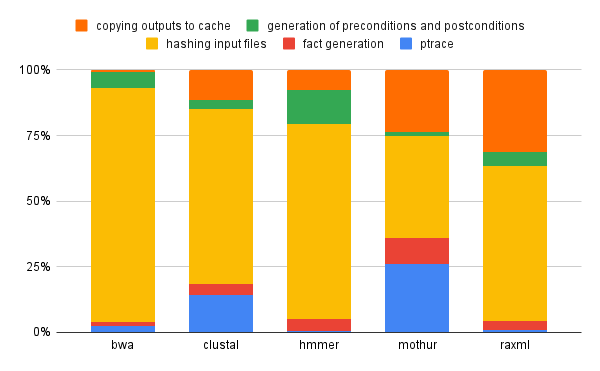
\includegraphics[width=0.7\textwidth]{component_overhead_breakdown.png}
\caption{\label{fig:component_overhead_breakdown} Percentage overhead breakdown of each of the different components which comprise \pc for each  bioinformatics workflows. The most obvious source of overhead is hashing input files, followed by copying output files to the cache.}
\end{figure}

\begin{figure}[ht]
\centering
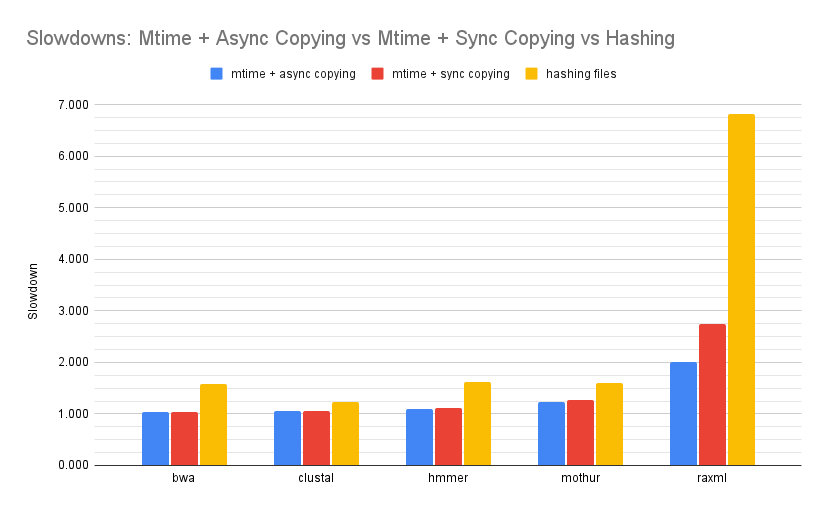
\includegraphics[width=0.7\textwidth]{slowdowns.png}
\caption{\label{fig:pc_slowdowns} Slowdown (normalized to baseline execution) for each bioinformatics workflow. The blue bars indicate the slowdown over baseline of running under \pc with the \texttt{mtime} checking mechanism and copying outputs files to the cache asynchronously (one background thread). The red bars indicate the slowdown over baseline of running under \pc with the \texttt{mtime} checking mechanism and copying output files to the cache synchronously. The yellow bars indicate the slowdown overbaseline of running under \pc with hashing input files as the checking mechanism and copying output files to the cache synchronously. Lower is better.}
\end{figure}

It becomes quickly apparent that \pc is spending an exorbitant amount of time hashing input files, and is doing so in every baseline. The reason \pc is hashing input files is to provide a precondition for the program; \pc  hashes the input file before the process actually opens it, in case the process modifies it. This has to be done at that time, and cannot be offloaded to some background task, or the wrong version of the contents of the file can be hashed. But, as we can tell, the correctness of hashing comes at a steep cost.

In order to work around the limitations of hashing, two solutions were proposed: copying the input files to the cache, and checking the \texttt{mtime} of the resource instead of hashing it. Neither of these is perfect. Copying the files to the cache provides moderate improvement, but does not provide the performance gains we are looking for, and also adds to the space that the cache requires. Using the \texttt{mtime} mechanism provides much better speedups, and so was incorporated into the system as an option. Checking the \texttt{mtime} is fragile, and is not a portable solution. Luckily, \pc can be run using whichever of these metrics the user chooses, depending on what they value most. The \texttt{mtime} checking mechanism provides quite a performance boost, but the \texttt{RAxML} workload, which has the most output files (by a significant margin) of the bioinformatics workflows, still has an overhead of 2.7x (see the \textbf{mtime + sync copying} results in Figure \ref{fig:pc_slowdowns}).

The second worst offender when it comes to overhead is the component of \pc that copies the output files to the cache. In the original \pc prototype, this was done at each process exit; this means that \pc is effectively blocked (and so are all the executions it is tracing) until it finishes copying the output files to the cache. Fortunately, unlike hashing input files, copying output files can be moved off the critical path. Because \pc has basic assumptions about how processes modifying the same file behave (Section \ref{sec:limitations}), and because output files are not copied to the cache until the end of execution, output files can be copied to the cache by background threads. A rudimentary experiment with just one background thread shows promising results (Figure \ref{fig:pc_slowdowns}. We plan to increase the number of parallel background threads copying output files to the cache and incorporate this into the system to improve the performance even more.
